\section{Attachements}
\subsection{Vorbereitung}
\subsubsection{Attachement A}

\subsubsection{Attachement B}

\subsubsection{Attachement D}

\subsubsection{Attachement E}

\subsection{Lowpass filter}
\subsubsection{Attachement F}

	\begin{figure}[h]
		\centering
		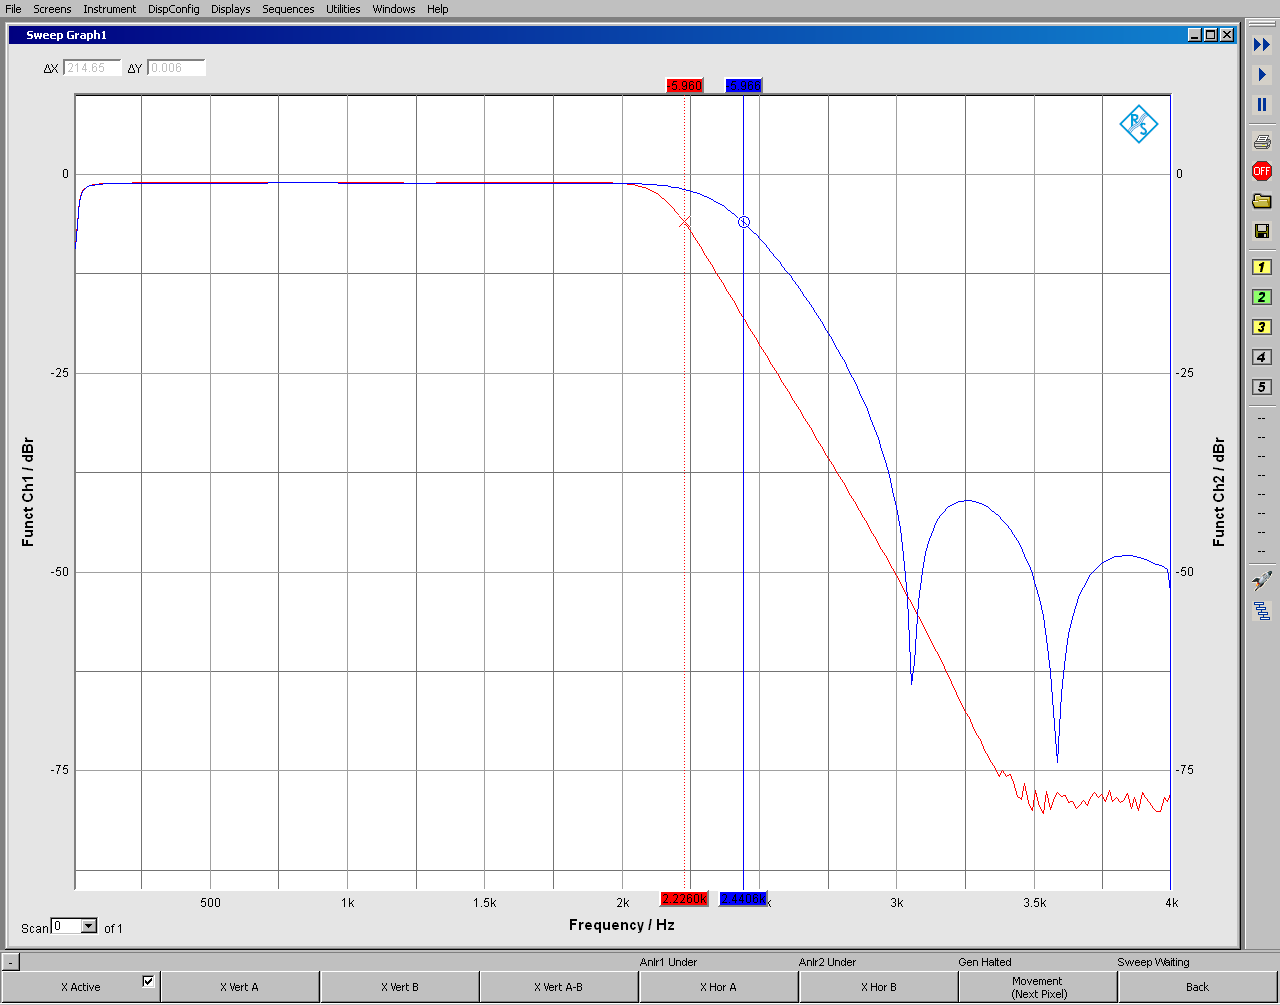
\includegraphics[width=0.8\linewidth]{Bilder/EllipCheby}
		\caption{Blau: Elliptisches IIR TP-Filter | Rot: Chebychev IIR TP-Filter}
		\label{fig:EllipCheby}
	\end{figure}

\subsubsection{Attachement G}

\subsection{Hochpass - Tiefpass - Weichenfilter}

\subsection{Modifiziertes elliptisches Tiefpassfilter}
\subsubsection{Attachement H}

\subsubsection{Attachement J}

\subsubsection{Attachement K}

	\begin{figure}[h]
		\centering
		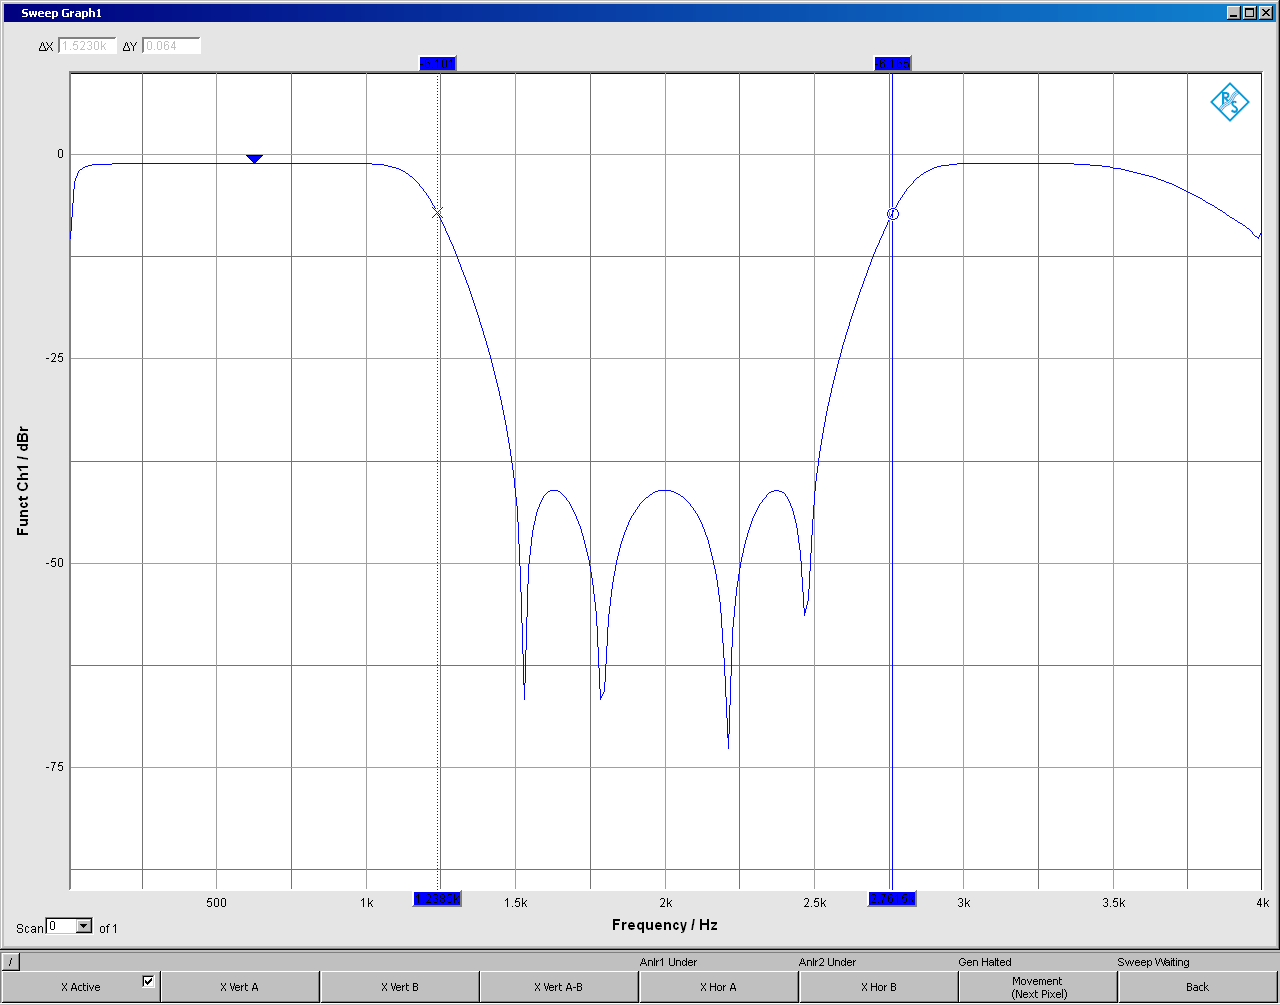
\includegraphics[width=0.7\linewidth]{Bilder/ellip2T}
		\caption{Frequenzgang modifiziertes Tiefpassfilter $|T| \rightarrow |2T|$}
		\label{fig:ellip2T}
	\end{figure}
